\documentclass[10pt, a4paper]{article} % 设置字体大小和纸张类型
\usepackage{fontspec}
\setmainfont{Times New Roman}

\usepackage{booktabs} % 支持更专业的表格线条
\usepackage{ctex}
\usepackage{caption} % 插图和表格的标题格式
\usepackage{amsmath, amsfonts, amssymb} % 数学公式支持
\usepackage{graphicx} % 插入图片
\usepackage{hyperref} % 超链接支持
\usepackage{hypcap} % 修正超链接指向的图片位置
\usepackage{geometry}
\usepackage{titlesec}
\usepackage{fmtcount} % 用于数字到中文的转换
\usepackage{enumitem} % 加载 enumitem 宏包
\usepackage{multirow} % 支持多行单元格
\usepackage{diagbox}
\usepackage{makecell} % 支持单元格内换行
\usepackage{tikz}
\usepackage{booktabs} % 支持更专业的表格线条
\usepackage{multirow} % 支持多行单元格
\usepackage{makecell}
\usepackage{unicode-math}
\setmathfont{Latin Modern Math}
\geometry{a4paper, margin=1.5cm} % 设置页边距

\renewcommand{\thesection}{\chinese{section}、}
\renewcommand{\thesubsection}{\arabic{subsection}.}


\begin{document}

\begin{titlepage}
    \newgeometry{left=0cm, right=0cm, top=0cm, bottom=0cm}
    \centering
    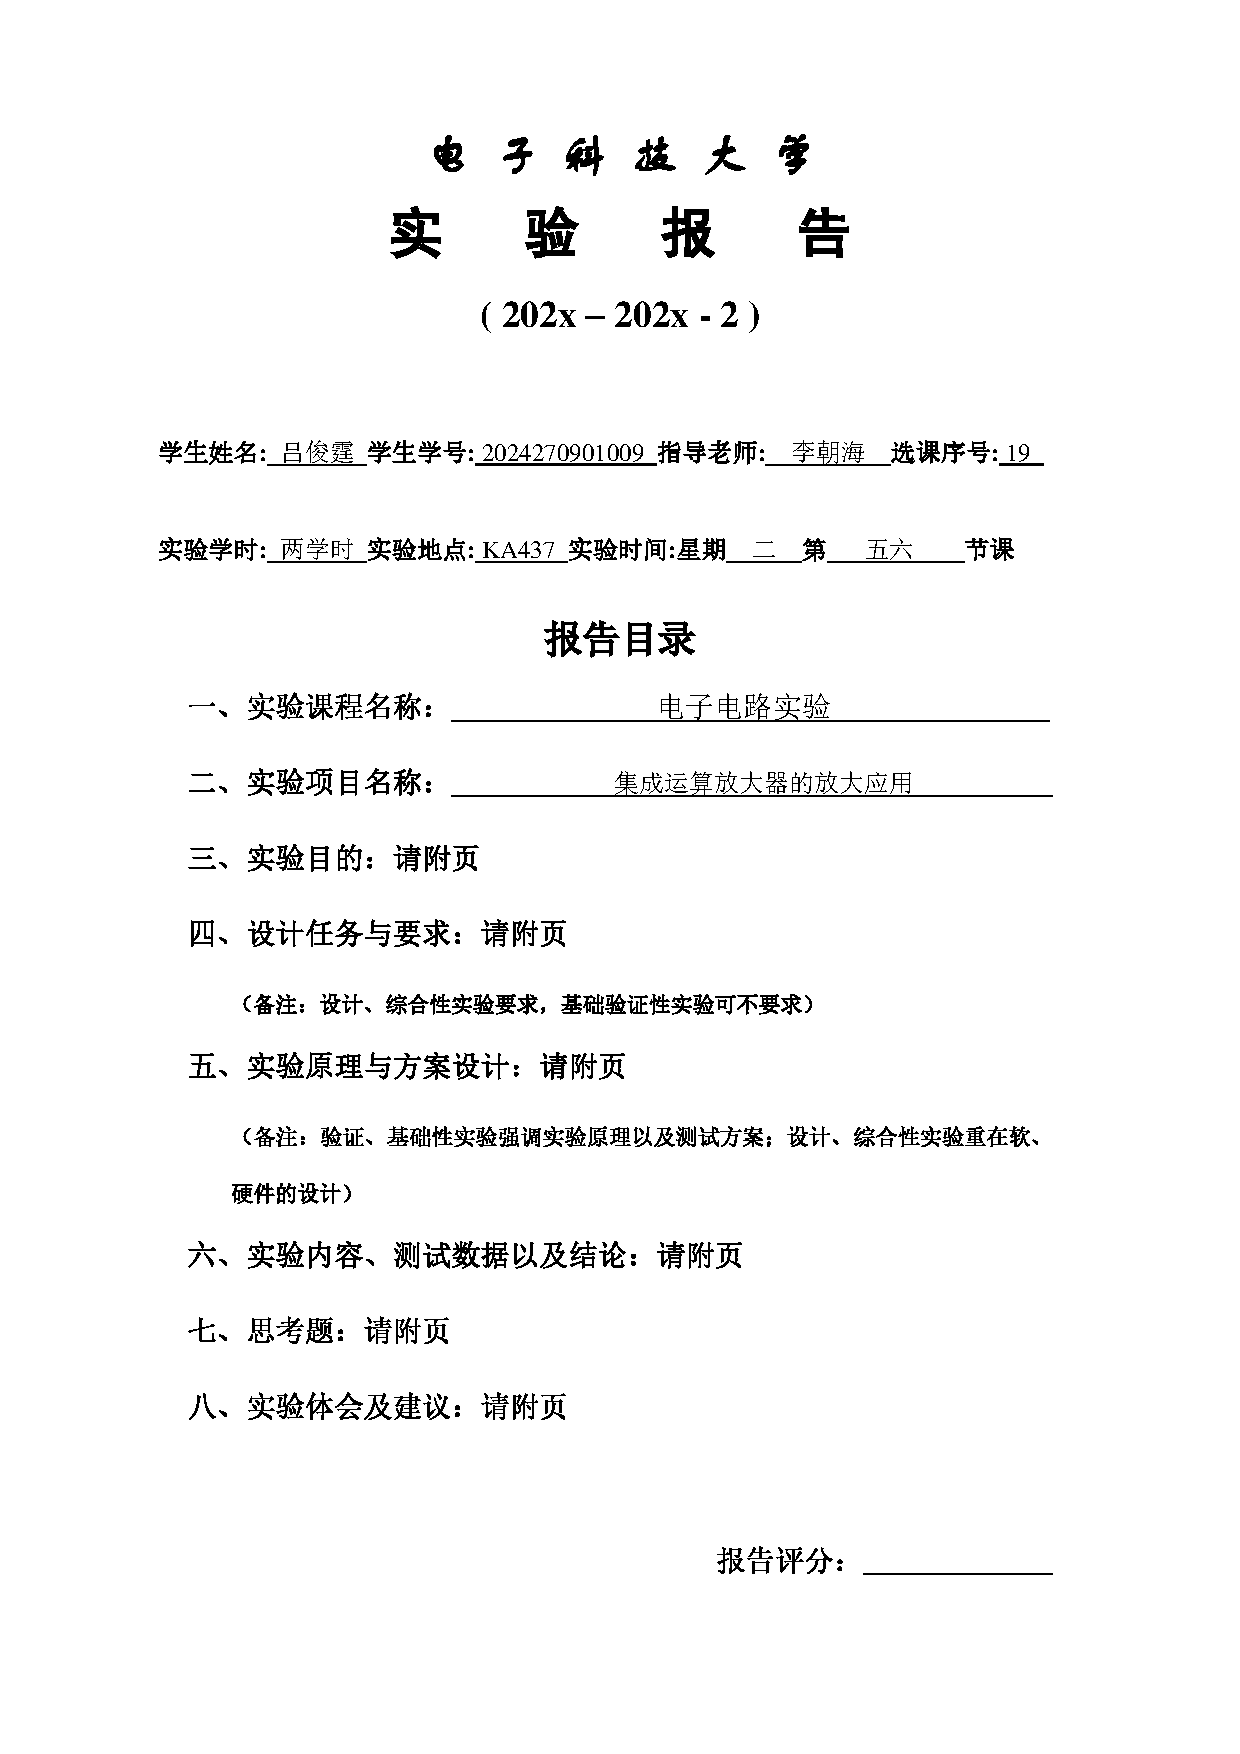
\includegraphics[page=1, width=0.9\textwidth, keepaspectratio]{image/实验报告撰写封面.pdf}
    \restoregeometry
\end{titlepage}

\setcounter{section}{2}

\section{实验目的}

\begin{enumerate}[leftmargin=50pt,label=(\arabic*)] % 设置序号格式为(1)
    \item 了解集成运算放大器的基础知识;
    \item 学习集成运算放大器的外部特性及使用方法;
    \item 理解集成运放构成的比例放大器原理。
\end{enumerate}

\section{设计任务与要求}

暂不需要。

\section{实验原理与方案设计}
\subsection{实验原理}
集成电路( IC )按功能可分为模拟集成电路和数字集成电路。模拟集成电路用来产生、放大和处理割裂连续变化的模拟量电信号。

集成运算放大器( OP ), 简称运放,是模拟集成电路中应用最广泛的一种,实质上是一种集成化的直接耦合式的多级放大器,具有高增益,高输入电阻、低输出电阻等特点。可以在负反馈之后对信号进行加减乘除积分微分指数对数等运算。
国际图形符号如图~\hyperref[fig:op_amp_symbol]{\ref{fig:op_amp_symbol}}所示。

\begin{figure}[ht]
    \centering
    \begin{minipage}{0.45\linewidth}
        \centering
        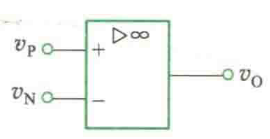
\includegraphics[width=\linewidth]{image/1.png}
        \caption{IEC国际标准符号}
        \label{fig:op_amp_symbol}
    \end{minipage}
    \hfill
    \begin{minipage}{0.45\linewidth}
        \centering
        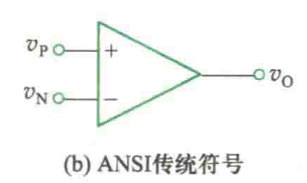
\includegraphics[width=\linewidth]{image/2.png}
        \caption{ANSI传统符号}
    \end{minipage}
\end{figure}


\section{实验内容、测试数据以及结论}
\subsection{实验内容}
\subsection{实验结论}
\section{思考题}
\subsection{题面}
\begin{enumerate}[leftmargin=50pt,label=(\arabic*)] % 设置序号格式为(1)
    \item 在BJT放大电路中, 直流电源的作用是什么? 如何设定放大器的静态工作点? 
    \item 影响放大器增益的主要因素有哪些? 
    \item 放大器输入电阻、输出电阻的物理意义是什么? 

\end{enumerate}
\subsection{回答}

\begin{enumerate}[leftmargin=50pt,label=(\arabic*)] % 设置序号格式为(1)
    \item 直流电源的作用是建立合适的静态工作点, 使得晶体管进入放大状态, 保证发射结正向偏置,集电结反向偏置还要使放大器能在正常放大的时候不会产生非线性失真。静态工作点一般选在适中的IC, 选小了容易出现小信号失真, 选大会出现饱和失真。
    \item 影响放大器增益的主要因素有晶体管的本身参数(如β、hfe等)、负载电阻、交流信号源内阻、偏置网络对信号的分压作用等。
    \item 放大器输入电阻是指在放大器输入端加上一个交流信号源时, 信号源看到的等效电阻。它反映了放大器对信号源的负载程度, 越大越好。输出电阻是指在放大器输出端接上一个负载时, 负载看到的等效电阻。它反映了放大器对负载的匹配程度, 越小越好。
\end{enumerate}

\section{实验体会及建议}
\subsection{实验体会}
测量时应注意小心调试仪器, 尽量将读数稳定在误差允许范围内进行读数。
\subsection{建议}
注意仪器正负极的接入, 防止反接造成仪器损坏。


\end{document}
